\chapter{Metodi tradizionali}
Se andiamo ad osservare gli algoritmi di codifica Lossy possiamo scomporli tutti in almeno tre blocchi principali. \cite{sadeeq2021image} \\
Un primo blocco si occupa di convertire l’immagine in una rappresentazione latente, tramite l’applicazione di una trasformata, in un altro dominio che permette di rappresentare l’informazione da comprimere in modo più sparso.\\
Successivamente si ha un blocco che si occupa di quantizzazione, ovvero di mappare i valori in ingresso in un insieme finito di dimensione più piccola rispetto a quello di ingresso. In questo passaggio so realizza la perdita di informazioni caratteristica della codifica Lossy.\\
Un ultimo blocco si occupa di effettuare la codifica entropica, in modo da comprimere ulteriormente l’informazione mappando i simboli usati più spesso con pochi bit.

\begin{figure}[ht]
    \centering
    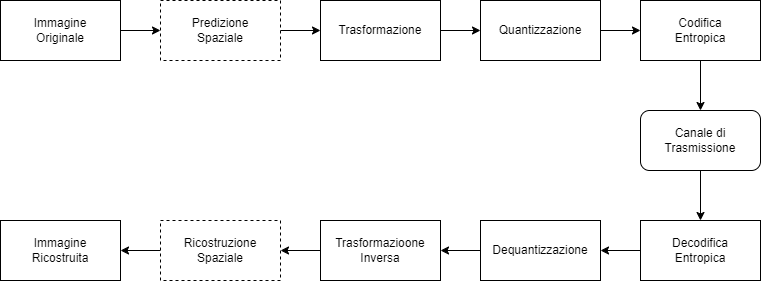
\includegraphics[width=0.8\textwidth]{Immagini/LossyCompressorDiagram.png}
    \caption{Diagramma di compressione Lossy}
    \label{fig:LossyCompressorDiagram}
\end{figure}

Gli algoritmi di compressione tradizionali usano trasformate statiche all’interno del primo blocco, messe a punto in numerosi anni di ricerca. Questa staticità non permette a questi metodi di adattarsi dinamicamente a tutti i tipi di contenuti delle immagini. \cite{cheng2018deep}  Inoltre rende il processo di sviluppo di un nuovo algoritmo di compressione un processo lungo che richiede anni di studi e progettazione. \cite{ cheng2018deep}
Andiamo ora a parlare brevemente dei metodi che andremo a considerare quando valuteremo le prestazioni dei vari algoritmi per poterli confrontare.

\section{JPEG}
Questo metodo di compressione sviluppato nel 1992 è diventato in poco tempo ed è attualmente il formato di compressione più diffuso. Nonostante in numerosi tentativi di sostituirlo con formati più moderni, questo è rimasto ancora ad oggi il formato più usato. Il JPEG si basa sull’utilizzo della DCT per realizzare la rappresentazione sparsificata dell’immagine originale. \cite{ 125072} \\
IMMAGINE CON JPEG

\section{JPEG2000}
Nel 2001 con la crescente diffusione di internet e con l’aumento di dimensione delle immagini e la richiesta di una maggiore qualità da parte degli utenti viene sviluppato questo nuovo formato chiamato appunto JPEG2000 per l’anno in cui è stato sviluppato.\\
JPEG2000 non utilizza la DCT come il suo predecessore ma vien introdotta una nuova trasformata la DWT o Discrete Wavelet Transformat che si propone di meglio identificare e comprimere i bordi delle figure che compongono le immagini. JPEG2000 quindi voleva essere un formato di qualità superiore con una compressione più efficiente. \cite{952804}
IMMAGINE CON JPEG2000

\section{BPG}
Questo formato è stato sviluppato da Fabrice Bellard nel 2014 come sostituto all’ormai affermato formato JPEG. Questo metodo di codifica si basa sulla codifica intra-frame del codec HEVC o H.265. \cite{BPGImageformat} Bellard voleva realizzare un formato molto leggero che potesse fornire immagini più compresse rispetto a JPEG, ma con una qualità superiore.\\
IMMAGINE CON BPG

\section{VVC}
Versatile Video Coding (VVC) o H.266 è lo standard di codifica video più recente, finalizzato nel luglio 2020. È stato sviluppato dal Joint Video Experts Team (JVET) dell'ITU-T Video Coding Experts Group (VCEG) e dell'ISO/IEC Moving Picture Experts Group (MPEG) per soddisfare la crescente richiesta di una migliore compressione video e per supportare una più ampia gamma di contenuti multimediali attuali e applicazioni emergenti come contenuti HDR, a 360°, per la Realtà Virtuale (VR) o la Realtà Aumentata (AR).\cite{9503377}\\
IMMAGINE CON VVC
